\part{Antiderivatives}

\chapter{The Indefinite Integral}

\section{The Indefinite Integral}

How do we undo a derivative? If we were given the derivative of a function $ f'(x) $, how could we find the original function $ f(x) $? The answer is called the antiderivative of $ f(x) $, which we will denote by the associated capital letter $ F(x) $. \\

Another way to think about this question is: "What function do I have to take the derivative of in order to get the answer?" The antiderivative of $ f(x) = 2x $ is $ x^2 $. \\

But what about $ F(x) = x^2 + 1 $? This works too! In fact, since when we take the derivative of a constant, we get zero. We could have chosen any constant. As a result, we report our antiderivative in its most general form $ x^2 + C $. The constant $ C $ is an important part of the antiderivative. \\

Notationally, we denote the operation of take the antiderivative (known as integration) as: \\

$$
    \int 2x \ dx = x^2 + C
$$

This is also called the indefinite integral of the function $ f(x) $, or sometimes just the integral of $ f(x) $, where $ f(x) $ is called the integrand. \\

That was a pretty simple example, so how do we find antiderivatives of more complicated expressions? In much the same way as we did with derivatives, we can generate a set of rules for finding antiderivatives, derived simply by thinking of our familiar derivative rules in reverse. \\

\section{Basic Antiderivative Rules}

The power rule for derivatives multiplies by the power and then subtracts one from the power. Reversing these operations means that we add one to the power and divide by the new power. \\

\subsection{Reverse Power Rule}

\begin{theorem}[Reverse Power Rule]
    \begin{align}
        \int x^n \ dx = {x^{n+1} \over n+1} + C,\ where\ n \ne -1
    \end{align}
\end{theorem}

\begin{exercise}\nonumber
    Find the anitiderivatives. \\

    (a)
    \begin{align}
         & \int x^6 \ dx \\
        \\
    \end{align}

    (b)
    \begin{align}
         & \int \sqrt[4]{t} \ dt \\
        \\
        \\
        \\
    \end{align}

    (c)
    \begin{align}
         & \int {1 \over x^{5/3}} \ dx \\
        \\
        \\
        \\
        \\
    \end{align}
\end{exercise}

\subsection{Antiderivative of Zero}

\begin{theorem}[Antiderivative of Zero]
    \begin{align}
        \int 0 \ dx = C
    \end{align}
\end{theorem}

\subsection{Antiderivative of a Constant}

\begin{theorem}[Antiderivative of a Constant]
    \begin{align}
        \int k \ dx = kx + C,\ where\ k\ is\ any\ constant
    \end{align}
\end{theorem}

\begin{exercise}\nonumber
    Find the anitiderivatives.

    \begin{align}
         & \int \pi \ dx \\
        \\
    \end{align}
\end{exercise}

\subsection{Multiplicative Constants}

\begin{theorem}[Multiplicative Constantst]
    \begin{align}
        \int kf(x) \ dx = k \int f(x) \ dx
    \end{align}
\end{theorem}

\begin{exercise}\nonumber
    Find the anitiderivatives. \\

    (a)
    \begin{align}
         & \int 4x^7 \ dx \\
        \\
        \\
        \\
        \\
    \end{align}

    (b)
    \begin{align}
         & \int {\pi \over \sqrt{t}} \ dt \\
        \\
        \\
        \\
        \\
    \end{align}
\end{exercise}

\subsection{Sum / Difference}

\begin{theorem}[Sum / Difference]
    \begin{align}
        \int (f(x) \pm g(x)) \ dx = \int f(x) \ dx \pm \int g(x) \ dx
    \end{align}
\end{theorem}

\begin{exercise}\nonumber
    Find the anitiderivatives. \\

    (a)
    \begin{align}
         & \int (3x^2 + 5) \ dx \\
        \\
        \\
        \\
    \end{align}

    (b)
    \begin{align}
         & \int \left({1 \over x^3} - {2 \over x^2}\right) \ dx \\
        \\
        \\
        \\
        \\
    \end{align}
\end{exercise}

\subsection{Trigonometric Functions}

\begin{theorem}[Trigonometric Functions]
    \begin{align}
        \int sin(x) \ dx       & = -cos(x) + C \\
        \int cos(x) \ dx       & = sin(x) + C  \\
        \int csc^2(x) \ dx     & = -cot(x) + C \\
        \int sec^2(x) \ dx     & = tan(x) + C  \\
        \int sec(x)tan(x) \ dx & = sec(x) + C  \\
        \int csc(x)cot(x) \ dx & = -csc(x) + C
    \end{align}
\end{theorem}

\subsection{Exponential / Logarithmic}

\begin{theorem}[Exponential / Logarithmic]
    \begin{align}
        \int a^xln(a) \ dx         & = a^x + C      \\
        \int e^xln(e) \ dx         & = e^x + C      \\
        \int {1 \over xln(a)} \ dx & = log_a|x| + C \\
        \int {1 \over x} \ dx      & = ln|x| + C
    \end{align}
\end{theorem}

\begin{exercise}\nonumber
    Find the anitiderivatives. \\

    (a)
    \begin{align}
         & \int 4^xln(4) + 5e^x - {6 \over x} \ dx \\
        \\
    \end{align}

    (b)
    \begin{align}
         & \int 3^z \ dz \\
        \\
        \\
        \\
    \end{align}
\end{exercise}

Sometimes we need to manipulate the integral a little bit before we can apply the rules. \\

\begin{exercise}\nonumber
    Find the anitiderivatives. \\

    (a)
    \begin{align}
         & \int {2s^3 - 5s^4 \over 3s^2} \ ds \\
        \\
        \\
        \\
        \\
        \\
    \end{align}

    (b)
    \begin{align}
         & \int \left({1 \over x} + {1 \over x^2}\right)\left(3 + 2x^2\right) \ dx \\
        \\
        \\
        \\
        \\
        \\
    \end{align}
\end{exercise}

\chapter{Chain Rule in Reverse}

\section{Chain Rule in Reverse}

The derivative of $ f(u(x)) $ is $ f'(u(x))u'(x) $, so \\

\begin{theorem}[Chain Rule in Reverse]
    \begin{align}
        \int f'(u(x))u'(x) \ dx = f(u(x)) + C
    \end{align}
\end{theorem}

Notice that in the integration, the $ u'(x) $ piece disappears, being absorbed back into $ f(x) $. The steps for finding the antiderivative of composition functions are as follows: \\

\begin{enumerate}
    \item
          Identify the core layer $ u(x) $. \\

    \item
          Identify the derivative of the core layer $ u'(x) $. \\

    \item
          Identify the outer layer $ f' $, and integrate $ f' $ leaving $ u(x) $ inside. \\
\end{enumerate}

\begin{exercise}\nonumber
    Find the anitiderivatives. \\

    (a)
    \begin{align}
         & \int (6x^2 + 1)sin(2x^3 + x) \ dx \\
        \\
        \\
        \\
        \\
        \\
        \\
        \\
    \end{align}

    (b)
    \begin{align}
         & \int sec^2(4t) \ dt \\
        \\
        \\
        \\
        \\
        \\
        \\
        \\
        \\
        \\
        \\
    \end{align}

    (c)
    \begin{align}
         & \int 4x^3(3x^4 - 1)^{14} \ dx \\
        \\
        \\
        \\
        \\
        \\
        \\
        \\
        \\
        \\
        \\
        \\
    \end{align}

    (d)
    \begin{align}
         & \int {e^{1 \over x} \over 4x^2} \ dx \\
        \\
        \\
        \\
        \\
        \\
        \\
        \\
        \\
        \\
        \\
        \\
    \end{align}
\end{exercise}

\begin{exercise}\nonumber
    Integrate in one step. \\

    \begin{align}
         & \int e^{-2t} + sin(3t) + cos\left({1 \over 4}t\right) \ dt \\
        \\
        \\
    \end{align}
\end{exercise}

\chapter{The Method of Substitution}

\section{The Method of Substitution}

The idea behind the method of substitution is to change a difficult integral in terms of one variable into an easier integral in terms of some other variable using a substitution. \\

\begin{theorem}[The Method of Substitution]
    \begin{align}
        \int f'(u(x)) \ {du \over dx} = \int f'(u) \ du
    \end{align}
\end{theorem}

\begin{exercise}\nonumber
    The method of substitution.

    \begin{align}
        \int (6x + 4)(3x^2 + 4x)^5 \ dx
    \end{align}

    \begin{enumerate}
        \item
              Identify the core layer $ u(x) = 3x^2 +4x $. \\

        \item
              Find the derivative of the core $ {du \over dx} = 6x + 4 $. \\

        \item
              Transform from an integral in $ x $ to an integral in the new variable $ u $ using the change of variable theorem. \\
              \begin{align}
                   & \int (6x + 4)(3x^2 + 4x)^5 \ dx \\
                   & = \int {du \over dx}u^5 \ dx    \\
                   & = \int u^5 \ du                 \\
                   & = {u^6 \over 6} + C
              \end{align}

        \item
              Convert back to the original variable by substituting $ u(x) $ back in.
              \begin{align}
                   & {u^6 \over 6} + C             \\
                   & = {(3x^2 + 4x)^6 \over 6} + C
              \end{align}
    \end{enumerate}
\end{exercise}

\begin{exercise}\nonumber
    Calculate using the method of substitution. \\

    (a)
    \begin{align}
         & \int sin(x)e^{5cos(x)} \ dx \\
        \\
        \\
        \\
        \\
        \\
        \\
        \\
        \\
        \\
        \\
        \\
        \\
        \\
        \\
        \\
    \end{align}

    (b)
    \begin{align}
         & \int {x \over (5x + 7)^3} \ dx \\
        \\
        \\
        \\
        \\
        \\
        \\
        \\
        \\
        \\
        \\
        \\
        \\
        \\
        \\
        \\
        \\
        \\
        \\
        \\
        \\
    \end{align}

    (c)
    \begin{align}
         & \int xsec(3x^2)tan(3x^2) \ dx \\
        \\
        \\
        \\
        \\
        \\
        \\
        \\
        \\
    \end{align}

    (d)
    \begin{align}
         & \int {-{1 \over t^2} + 1 \over \sqrt{{1 \over t} + t}} \ dt \\
        \\
        \\
        \\
        \\
        \\
        \\
        \\
        \\
        \\
        \\
        \\
        \\
        \\
        \\
        \\
    \end{align}

    (e)
    \begin{align}
         & \int (1 + 900x)^{1/15000} \ dx \\
        \\
        \\
        \\
        \\
        \\
        \\
        \\
        \\
        \\
        \\
    \end{align}

    (f)
    \begin{align}
         & \int sin(\theta)(cos^3\theta - cos^5\theta) \ d\theta \\
        \\
        \\
        \\
    \end{align}

    (g)
    \begin{align}
         & \int {7x \over 4x^2 + 9} \ dx \\
        \\
        \\
        \\
        \\
        \\
        \\
        \\
        \\
        \\
        \\
        \\
        \\
        \\
    \end{align}

    (h)
    \begin{align}
         & \int (2x + 5) \cdot \sqrt[3]{3x + 1} \ dx \\
        \\
        \\
        \\
        \\
        \\
        \\
        \\
        \\
        \\
        \\
        \\
        \\
        \\
        \\
        \\
        \\
        \\
        \\
        \\
        \\
        \\
        \\
        \\
        \\
        \\
        \\
    \end{align}
\end{exercise}

\chapter{Definite Integrals}

\section{Riemann Sum}

Suppose we wanted to find the area underneath the graph of a straight line that lies above the x-axis, between $ x = a $ and $  x = b $. Since we have formulas for finding the area of basic shapes, we can easily figure this out. \\

\begin{figure}[H]
    \centering
    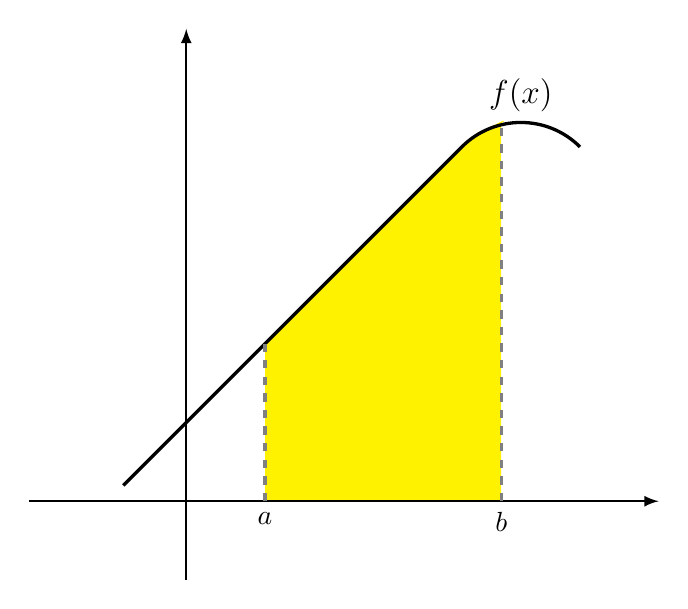
\begin{tikzpicture}
        \fill[yellow](1,0) -- (1,2) -- (3.5,4.5) to[out=45,in=35] (4,4.8) -- (4,0) -- cycle;
        \draw[thick,-latex] (-2,0) -- (6,0);
        \draw[thick,-latex] (0,-1) -- (0,6);
        \draw[very thick,black] (-0.8,0.2) -- (3.5,4.5) to[out=45,in=135] node[pos=0.5,above,font=\large]{$ f(x) $} (5,4.5);
        \draw[very thick,dashed,gray]
        (1,0) node[below,black] {$a$} -- (1,2)
        (4,0) node[below,black] {$b$} -- (4,4.8);
    \end{tikzpicture}
\end{figure}

But what about finding the area underneath the graph of a general curve $ y = f(x) $ and above the x-axis between $  x = a $ and $ x = b $? \\

Bernhard Riemann's idea was to carve up the desired area into rectangle and user their area to estimate the true area. He called this the Riemann Sum and it goes as follows: \\

\begin{enumerate}
    \item
          Create a partition $ P $, dividing up the interval $ [a, b] $ into n subintervals $ I_1, I_2, \dots, I_n $. \\

    \item
          Choose an x-value (called it $ x_k $) in each subinterval $ I_k $. \\

    \item
          For each $ x_k $ we choose, draw a rectangle with height $ f(x_k) $ and a width spanning $ I_k $ ($ \Delta x_k $). \\
\end{enumerate}

\begin{figure}[H]
    \centering
    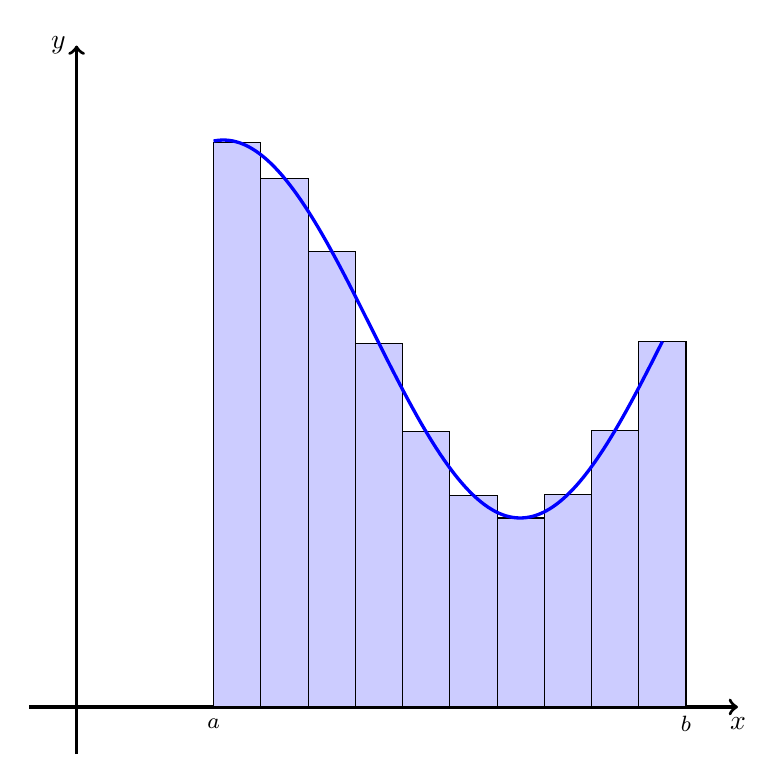
\begin{tikzpicture}[scale=1.2]
        \def\a{1.7}
        \def\b{5.7}
        \def\c{3.7}
        \def\L{0.5} % width of interval

        \pgfmathsetmacro{\Va}{2*sin(\a r+1)+4} \pgfmathresult
        \pgfmathsetmacro{\Vb}{2*sin(\b r+1)+4} \pgfmathresult
        \pgfmathsetmacro{\Vc}{2*sin(\c r+1)+4} \pgfmathresult

        \draw[->,very thick] (-0.5,0) -- (7,0) coordinate (x axis) node[below] {$x$};
        \draw[->,very thick] (0,-0.5) -- (0,7) coordinate (y axis) node[left] {$y$};
        \foreach \f in {1.7,2.2,...,6.2} {\pgfmathparse{2*sin(\f r+1)+4} \pgfmathresult
                \draw[fill=blue!20] (\f-\L/2,\pgfmathresult |- x axis) -- (\f-\L/2,\pgfmathresult) -- (\f+\L/2,\pgfmathresult) -- (\f+\L/2,\pgfmathresult |- x axis) -- cycle;}
        \node at (\a-\L/2,-5pt) {\footnotesize{$a$}};
        \node at (\b+\L/2+\L,-5pt) {\footnotesize{$b$}};
        \draw[blue,very thick,smooth,samples=100,domain=1.45:6.2] plot(\x,{2*sin(\x r+1)+4});
    \end{tikzpicture}
\end{figure}

The area of rectangle $ k $ is:
$$
    f(x_k) \cdot \Delta x_k
$$

The total area of all the rectangles is:
$$
    f(x_1) \cdot \Delta x_1 + f(x_2) \cdot \Delta x_2 + \dots + f(x_n) \cdot \Delta x_n = \sum_{k=1}^{n} f(x_k) \cdot \Delta x_k
$$

\begin{exercise}\nonumber
    Use the Riemann Sum to estimate the area below $ y = sin({1 \over 2}x) $ and above the x-axis, between $ x = 0 $ and $ x = 2\pi $. Use a partition of 4 subintervals. \\

    \begin{figure}[H]
        \centering
        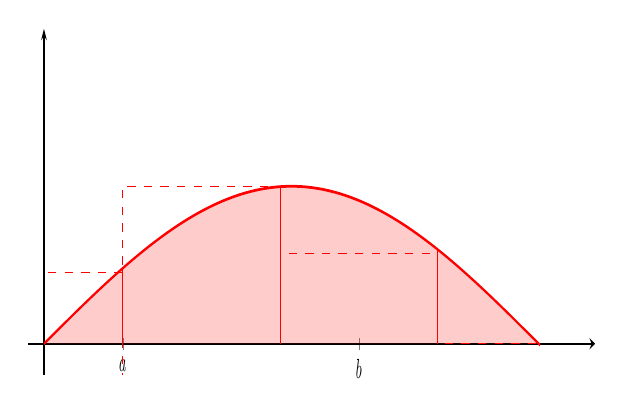
\begin{tikzpicture}[
                declare function={
                        f(\x)=sin(deg(0.5*\x));
                    },
                xscale=0.5
            ]
            \begin{axis}[
                    axis lines = middle,
                    xtick ={1,4},
                    ytick ={0},
                    xticklabels = {$a$,$b$},
                    ymin = -0.2,
                    ymax = 2,
                    xmin = -0.2,
                    xmax = 7,
                    x=2cm,y=2cm,
                    axis line style = thick,
                ]

                \addplot [
                    domain=0:6.3,
                    samples=300,
                    line width=1pt,
                    fill=red, draw=none,
                    fill opacity=0.2
                ] {f(x)} \closedcycle;

                \addplot [
                    domain=0:6.3,
                    samples=300,
                    line width = 1pt, red
                ] {f(x)};

                \addplot [
                    ycomb, thick, red,
                    no markers,
                    samples at={1,3,5}
                ] {f(x)};
            \end{axis}
            \draw[dashed,red] (2.4, 1.3) -- (0.3, 1.3);
            \draw[dashed,red] (6.1, 2.4) -- (2.4, 2.4) -- (2.4, 0);
            \draw[dashed,red] (10.2, 1.55) -- (6.4, 1.55);
            \draw[dashed,red] (12.9, 0.4) -- (10.4, 0.4);
        \end{tikzpicture}
    \end{figure}

    \begin{align}
        \\
        \\
        \\
        \\
        \\
        \\
        \\
        \\
    \end{align}
\end{exercise}

So, what happens as make the rectangles skinnier? \\

\begin{figure}[H]
    \centering
    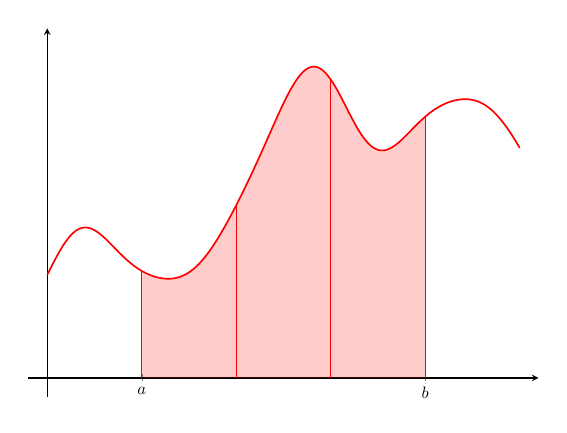
\begin{tikzpicture}[scale=0.6,
            declare function={
                    f(\x)=2+sin(deg(\x-2))+sin(deg(3*\x))/2+sin(deg(5*\x))/8 + sin(deg(7*\x))/28;
                }
        ]
        \begin{axis}[
                axis lines = middle,
                xtick ={1,4},
                ytick ={0},
                xticklabels = {$a$,$b$},
                ymin = -0.2,
                ymax = 3.7,
                xmin = -0.2,
                xmax = 5.2,
                x=2cm,y=2cm,
                axis line style = thick,
            ]

            \addplot [
                domain=1:4,
                samples=300,
                line width=1pt,
                fill=red, draw=none,
                fill opacity=0.2
            ] {f(x)} \closedcycle;

            \addplot [
                domain=0:5,
                samples=300,
                line width = 1pt, red
            ] {f(x)};

            \addplot [
                ycomb, thick, red,
                no markers,
                samples at={1,2,...,4}
            ] {f(x)};
        \end{axis}
    \end{tikzpicture}
\end{figure}

\begin{figure}[H]
    \centering
    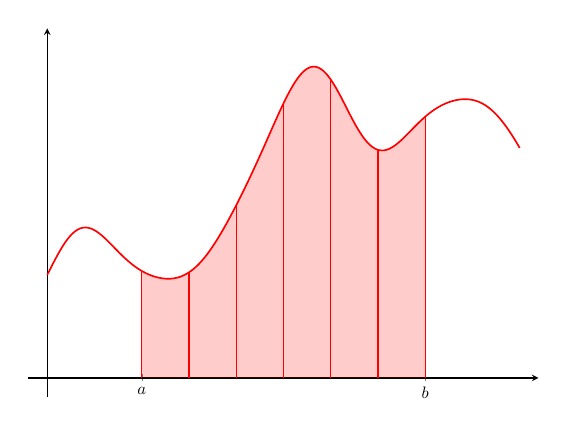
\begin{tikzpicture}[scale=0.6,
            declare function={
                    f(\x)=2+sin(deg(\x-2))+sin(deg(3*\x))/2+sin(deg(5*\x))/8 + sin(deg(7*\x))/28;
                }
        ]
        \begin{axis}[
                axis lines = middle,
                xtick ={1,4},
                ytick ={0},
                xticklabels = {$a$,$b$},
                ymin = -0.2,
                ymax = 3.7,
                xmin = -0.2,
                xmax = 5.2,
                x=2cm,y=2cm,
                axis line style = thick,
            ]

            \addplot [
                domain=1:4,
                samples=300,
                line width=1pt,
                fill=red, draw=none,
                fill opacity=0.2
            ] {f(x)} \closedcycle;

            \addplot [
                domain=0:5,
                samples=300,
                line width = 1pt, red
            ] {f(x)};

            \addplot [
                ycomb, thick, red,
                no markers,
                samples at={1,1.5,...,4}
            ] {f(x)};
        \end{axis}
    \end{tikzpicture}
\end{figure}

\begin{figure}[H]
    \centering
    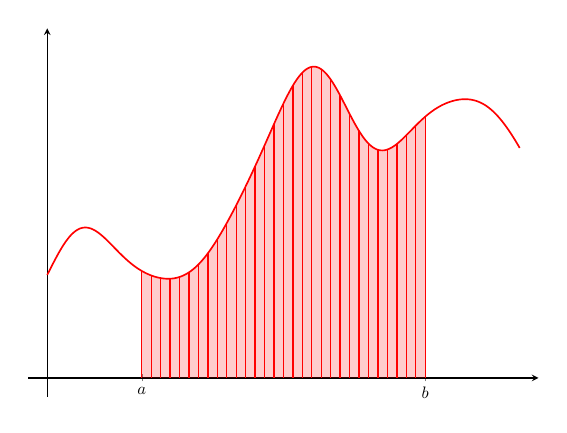
\begin{tikzpicture}[scale=0.6,
            declare function={
                    f(\x)=2+sin(deg(\x-2))+sin(deg(3*\x))/2+sin(deg(5*\x))/8 + sin(deg(7*\x))/28;
                }
        ]
        \begin{axis}[
                axis lines = middle,
                xtick ={1,4},
                ytick ={0},
                xticklabels = {$a$,$b$},
                ymin = -0.2,
                ymax = 3.7,
                xmin = -0.2,
                xmax = 5.2,
                x=2cm,y=2cm,
                axis line style = thick,
            ]

            \addplot [
                domain=1:4,
                samples=300,
                line width=1pt,
                fill=red, draw=none,
                fill opacity=0.2
            ] {f(x)} \closedcycle;

            \addplot [
                domain=0:5,
                samples=300,
                line width = 1pt, red
            ] {f(x)};

            \addplot [
                ycomb, thick, red,
                no markers,
                samples at={1,1.1,...,4}
            ] {f(x)};
        \end{axis}
    \end{tikzpicture}
\end{figure}

As the width of the rectangles decreases, the accuracy of the estimate increases. So, what happens if we let the width of all the rectangles in the partition approach 0? \\

Notationally:

$$
    \lim\limits_{\substack{n \rightarrow \infty \\ \left\|p\right\| \rightarrow 0}} \sum_{k=1}^{n} f(x_k) \cdot \Delta x_k
$$

We should get the exact area, that is, our estimate is no longer just an estimate. \\

Notationally, instead of limit, we write it as: \\

\begin{theorem}[Definite Integral]
    \begin{align}
        \int_{x = a}^{b} f(x) \ dx
    \end{align}
\end{theorem}

\section{Definite Integral}

For all of the following, suppose that $ k $, $ a $, $ b $, and $ c $ are constants with $ a < b < c $, and that $ f $ and $ g $ are integrable functions on the domain of integration. \\

\begin{theorem}[Definite Integral]
    \begin{align}
        \int_a^b k \ dx = (b - a)k
    \end{align}
\end{theorem}

\begin{figure}[H]
    \centering
    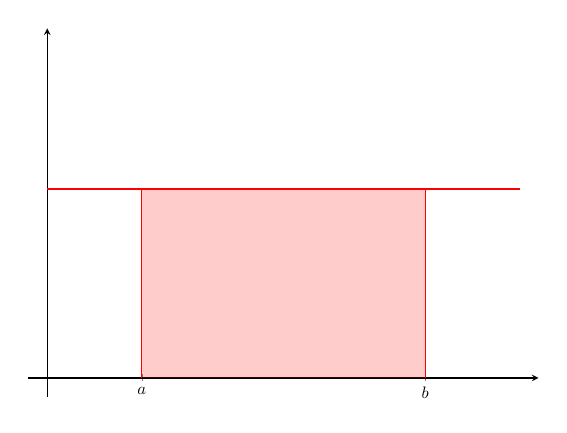
\begin{tikzpicture}[scale=0.6,
            declare function={
                    f(\x)=2;
                }
        ]
        \begin{axis}[
                axis lines = middle,
                xtick ={1,4},
                ytick ={0},
                xticklabels = {$a$,$b$},
                ymin = -0.2,
                ymax = 3.7,
                xmin = -0.2,
                xmax = 5.2,
                x=2cm,y=2cm,
                axis line style = thick,
            ]

            \addplot [
                domain=1:4,
                samples=300,
                line width=1pt,
                fill=red, draw=none,
                fill opacity=0.2
            ] {f(x)} \closedcycle;

            \addplot [
                domain=0:5,
                samples=300,
                line width = 1pt, red
            ] {f(x)};

            \addplot [
                ycomb, thick, red,
                no markers,
                samples at={1,4}
            ] {f(x)};
        \end{axis}
    \end{tikzpicture}
\end{figure}

\begin{theorem}[Definite Integral]
    \begin{align}
        \int_a^a f(x) \ dx = 0
    \end{align}
\end{theorem}

\begin{figure}[H]
    \centering
    \begin{tikzpicture}[scale=0.6,
            declare function={
                    f(\x)=0.5 * sin(deg(\x)) + 2;
                }
        ]
        \begin{axis}[
                axis lines = middle,
                xtick ={1},
                ytick ={0},
                xticklabels = {$a$},
                ymin = -0.2,
                ymax = 3.7,
                xmin = -0.2,
                xmax = 5.2,
                x=2cm,y=2cm,
                axis line style = thick,
            ]

            \addplot [
                domain=0:5,
                samples=300,
                line width = 1pt, red
            ] {f(x)};

            \addplot [
                ycomb, thick, red,
                no markers,
                samples at={1}
            ] {f(x)};
        \end{axis}
    \end{tikzpicture}
\end{figure}

\begin{theorem}[Definite Integral]
    \begin{align}
        \int_b^a f(x) \ dx = -\int_a^b f(x) \ dx
    \end{align}
\end{theorem}

\begin{figure}[H]
    \centering
    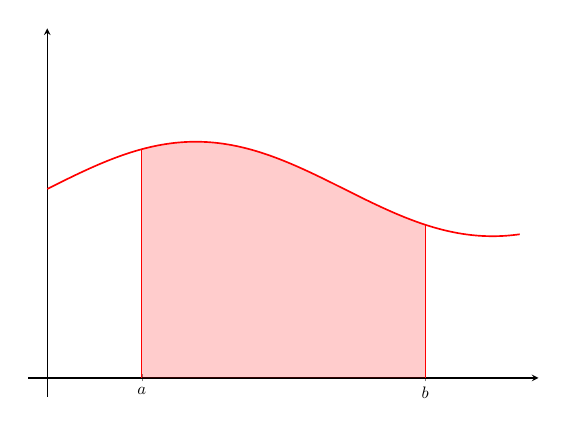
\begin{tikzpicture}[scale=0.6,
            declare function={
                    f(\x)=0.5 * sin(deg(\x)) + 2;
                }
        ]
        \begin{axis}[
                axis lines = middle,
                xtick ={1,4},
                ytick ={0},
                xticklabels = {$a$,$b$},
                ymin = -0.2,
                ymax = 3.7,
                xmin = -0.2,
                xmax = 5.2,
                x=2cm,y=2cm,
                axis line style = thick,
            ]

            \addplot [
                domain=1:4,
                samples=300,
                line width=1pt,
                fill=red, draw=none,
                fill opacity=0.2
            ] {f(x)} \closedcycle;

            \addplot [
                domain=0:5,
                samples=300,
                line width = 1pt, red
            ] {f(x)};

            \addplot [
                ycomb, thick, red,
                no markers,
                samples at={1,4}
            ] {f(x)};
        \end{axis}
    \end{tikzpicture}
\end{figure}

\begin{theorem}[Definite Integral]
    \begin{align}
        \int_a^c f(x) \ dx = \int_a^b f(x) \ dx + \int_b^c f(x) \ dx
    \end{align}
\end{theorem}

\begin{figure}[H]
    \centering
    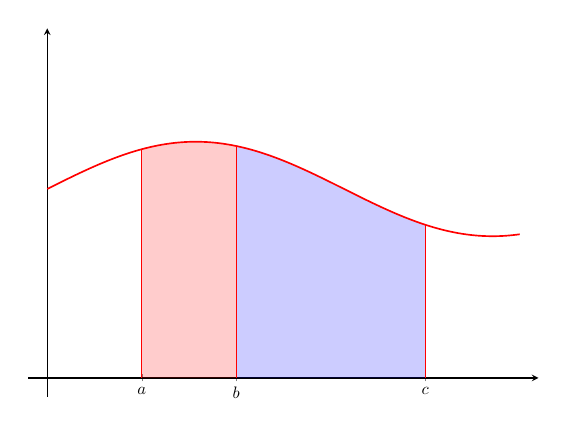
\begin{tikzpicture}[scale=0.6,
            declare function={
                    f(\x)=0.5 * sin(deg(\x)) + 2;
                }
        ]
        \begin{axis}[
                axis lines = middle,
                xtick ={1,2,4},
                ytick ={0},
                xticklabels = {$a$,$b$,$c$},
                ymin = -0.2,
                ymax = 3.7,
                xmin = -0.2,
                xmax = 5.2,
                x=2cm,y=2cm,
                axis line style = thick,
            ]

            \addplot [
                domain=1:2,
                samples=300,
                line width=1pt,
                fill=red, draw=none,
                fill opacity=0.2
            ] {f(x)} \closedcycle;

            \addplot [
                domain=2:4,
                samples=300,
                line width=1pt,
                fill=blue, draw=none,
                fill opacity=0.2
            ] {f(x)} \closedcycle;

            \addplot [
                domain=0:5,
                samples=300,
                line width = 1pt, red
            ] {f(x)};

            \addplot [
                ycomb, thick, red,
                no markers,
                samples at={1,2,4}
            ] {f(x)};
        \end{axis}
    \end{tikzpicture}
\end{figure}

\begin{theorem}[Definite Integral]
    \begin{align}
        \int_a^b kf(x) \ dx = k \int_a^b f(x) \ dx
    \end{align}
\end{theorem}

\begin{figure}[H]
    \centering
    \begin{tikzpicture}[scale=0.6,
            declare function={
                    f(\x)=0.5 * sin(deg(\x)) + 2;
                    g(\x)=0.5 * sin(deg(\x)) + 1;
                }
        ]
        \begin{axis}[
                axis lines = middle,
                xtick ={1,4},
                ytick ={0},
                xticklabels = {$a$,$b$},
                ymin = -0.2,
                ymax = 3.7,
                xmin = -0.2,
                xmax = 5.2,
                x=2cm,y=2cm,
                axis line style = thick,
            ]

            \addplot [
                domain=0:5,
                samples=300,
                line width = 1pt, red
            ] {f(x)};

            \addplot [
                domain=0:5,
                samples=300,
                line width = 1pt, red
            ] {g(x)};
        \end{axis}
    \end{tikzpicture}
\end{figure}

\begin{theorem}[Definite Integral]
    \begin{align}
        \int_a^b (f(x) \pm g(x))  \ dx = \int_a^b f(x) \ dx \pm \int_a^b g(x) \ dx
    \end{align}
\end{theorem}

\begin{figure}[H]
    \centering
    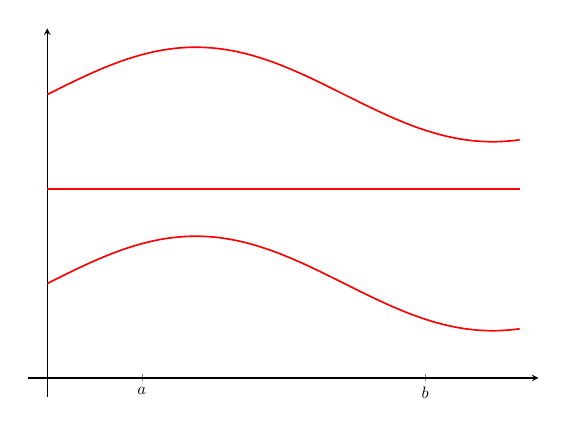
\begin{tikzpicture}[scale=0.6,
            declare function={
                    f(\x)=0.5 * sin(deg(\x)) + 1;
                    g(\x)=2;
                    h(\x)=0.5 * sin(deg(\x)) + 3;
                }
        ]
        \begin{axis}[
                axis lines = middle,
                xtick ={1,4},
                ytick ={0},
                xticklabels = {$a$,$b$},
                ymin = -0.2,
                ymax = 3.7,
                xmin = -0.2,
                xmax = 5.2,
                x=2cm,y=2cm,
                axis line style = thick,
            ]

            \addplot [
                domain=0:5,
                samples=300,
                line width = 1pt, red
            ] {f(x)};

            \addplot [
                domain=0:5,
                samples=300,
                line width = 1pt, red
            ] {g(x)};
            \addplot [
                domain=0:5,
                samples=300,
                line width = 1pt, red
            ] {h(x)};
        \end{axis}
    \end{tikzpicture}
\end{figure}

\begin{exercise}\nonumber
    Evaluate. \\

    (a)
    \begin{align}
         & \int_1^2 {1 \over t} \ dt \\
        \\
        \\
        \\
    \end{align}

    (b)
    \begin{align}
         & \int_{-2}^1 x^3 \ dx \\
        \\
        \\
        \\
        \\
        \\
        \\                   \\
    \end{align}

    (c)
    \begin{align}
         & \int_1^5 s(s^2 + 1) \ ds \\
        \\
        \\
        \\
        \\
        \\
        \\
        \\
        \\
    \end{align}

    (d)
    \begin{align}
        \int_{\sqrt{ln(2)}}^{\sqrt{ln(4)}} xe^{x^2} \ dx \\
        \\
        \\
        \\
        \\
        \\
        \\
        \\
        \\
        \\
        \\
        \\
        \\
        \\
        \\
        \\
    \end{align}

    (e)
    \begin{align}
         & \int_x^{x^2} sin(t) \ dt \\
        \\
        \\
        \\
        \\
        \\
    \end{align}

    (f)
    \begin{align}
        \int_5^{13} (x + 1)\sqrt{2x - 1} \ dx \\
        \\
        \\
        \\
        \\
        \\
        \\
        \\
        \\
        \\
        \\
        \\
        \\
        \\
        \\
        \\
        \\
        \\
        \\
        \\
        \\
        \\
        \\
        \\
        \\
        \\
        \\
        \\
        \\
    \end{align}
\end{exercise}

\chapter{Area Under a Curve}

\section{Area Under a Curve}

\begin{exercise}\nonumber
    Find the area below the curve $ f(x) = sin(x) $ and above the x-axis between $ x = {\pi \over 2} $ and $ x = \pi $. \\

    \begin{figure}[H]
        \centering
        \begin{tikzpicture}[scale=0.8,yscale=0.2]
            \draw[->] (-1,0) -- (8,0) node[right] {$ x $};
            \draw[->] (0,-10) -- (0,30) node[above] {$ y $};
            \draw[very thick,color=red,domain=-1:7] plot (\x,{-2 * (\x - 3.14) ^ 2 + 20});
            \draw[-,very thick,red] (3.14, 0) -- (3.14,20);
            \node at (1.5,-2) [] {$ \pi \over 4 $};
            \node at (3.14,-2) [] {$ \pi \over 2 $};
            \node at (4.8,-2) [] {$ 3\pi \over 4 $};
            \node at (6,-2) [] {$ \pi $};
        \end{tikzpicture}
    \end{figure}

    \begin{align}
        \\
        \\
        \\
        \\
        \\
        \\
    \end{align}
\end{exercise}

What if we have a more interesting situation where many curves are involved? For instance, how do we find the area between two curves $ f $ and $ g $? \\

\begin{figure}[H]
    \centering
    \begin{tikzpicture}
        \begin{axis}[
                xlabel={$x$},
                ylabel={$y$},
                xtick={-3,0,1},
                ytick={2},
                samples=100,
                domain=-4:1,
                xmin=-4,xmax=2,
                ymin=-1,ymax=3,
            ]
            \addplot[name path=func, red, very thick, mark=none, ] {sqrt(-x+1)};
            \addplot[name path=line, red, very thick] {2};
            \addplot fill between[
                    of = func and line,
                    soft clip={domain=-3:0},
                    every even segment/.style  = {gray,opacity=.4}
                ];
            \draw[thick,dashed,brown] (axis cs:-3,0) -- (axis cs:-3,2);
        \end{axis}
    \end{tikzpicture}
\end{figure}

$$
    \text{Area under Upper} - \text{Area under Lower} = \text{Area expected}
$$

\begin{exercise}\nonumber
    Calculate the area bounded by $ y = 2x + 1 $ and $ y = x^2 - 2x - 3 $. \\

    \begin{figure}[H]
        \centering
        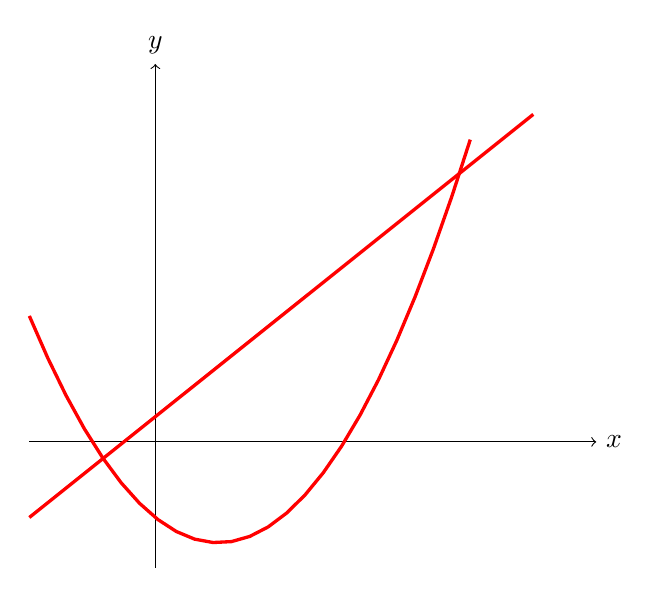
\begin{tikzpicture}[scale=0.8,yscale=0.4]
            \draw[->] (-2,0) -- (7,0) node[right] {$ x $};
            \draw[->] (0,-5) -- (0,15) node[above] {$ y $};
            \draw[very thick,color=red,domain=-2:6] plot (\x,{2 * (\x) + 1});
            \draw[very thick,color=red,domain=-2:5] plot (\x,{(\x) ^ 2 - 2 * \x - 3});
        \end{tikzpicture}
    \end{figure}

    \begin{align}
        \\
        \\
        \\
        \\
        \\
        \\
        \\
        \\
        \\
        \\
        \\
        \\
        \\
        \\
        \\
        \\
        \\
    \end{align}
\end{exercise}

\begin{exercise}\nonumber
    Calculate the area bounded by $ y = -x $, $ y = \sqrt{x} $, and $ y = -x^2 + 2 $ between $ x = 0 $ and $ x = 2 $. \\

    \begin{figure}[H]
        \centering
        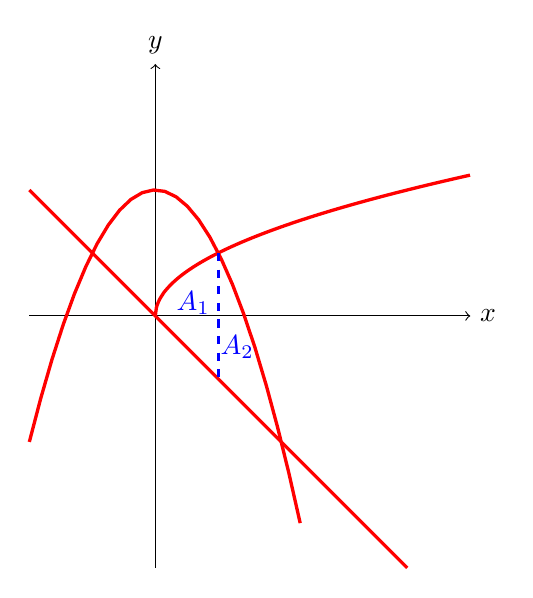
\begin{tikzpicture}[scale=0.8]
            \draw[->] (-2,0) -- (5,0) node[right] {$ x $};
            \draw[->] (0,-4) -- (0,4) node[above] {$ y $};
            \draw[very thick,color=red,domain=-2:4] plot (\x,{-(\x)});
            \draw[very thick,color=red,domain=0:5,samples=300] plot (\x,{\x ^ (1/2)});
            \draw[very thick,color=red,domain=-2:2.3] plot (\x,{-(\x) ^ 2 + 2});
            \draw[dashed, very thick,color=blue] (1, 1) -- (1, -1);
            \node at (0.6, 0.2) [blue] {$ A_1 $};
            \node at (1.3, -0.5) [blue] {$ A_2 $};
        \end{tikzpicture}
    \end{figure}

    \begin{align}
        \\
        \\
        \\
        \\
        \\
        \\
        \\
        \\
        \\
        \\
        \\
    \end{align}
\end{exercise}

\begin{exercise}\nonumber
    Find the area bounded by $ y^2 = x + 4 $ and $ y = {1 \over 2}x + {1 \over 2} $. \\

    \begin{figure}[H]
        \centering
        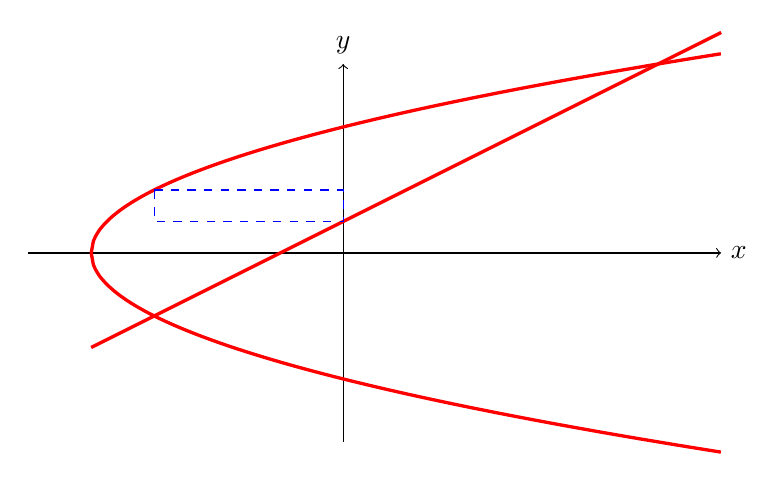
\begin{tikzpicture}[scale=0.8]
            \draw[->] (-5,0) -- (6,0) node[right] {$ x $};
            \draw[->] (0,-3) -- (0,3) node[above] {$ y $};
            \draw[very thick,color=red,domain=-4:6] plot (\x,{0.5 * \x + 0.5});
            \draw[very thick,color=red,domain=-4:6,samples=300] plot (\x,{(\x + 4) ^ (1/2)});
            \draw[very thick,color=red,domain=-4:6,samples=300] plot (\x,{-(\x + 4) ^ (1/2)});
            \draw[dashed,blue] (-3,1) -- (0,1) -- (0,0.5) -- (-3,0.5) -- (-3,1);
        \end{tikzpicture}
    \end{figure}

    \begin{align}
        \\
        \\
        \\
        \\
        \\
        \\
        \\
        \\
        \\
        \\
        \\
        \\
        \\
        \\
        \\
        \\
                                         \\
                                         \\
                                         \\
                                         \\
    \end{align}
\end{exercise}